\documentclass[MASTER.tex]{subfiles} 
\begin{document} 
%===========================================================
\begin{frame}
\huge
Important Components of the Python Scientific Stack
\end{frame}
\begin{frame}
	\begin{figure}
\centering
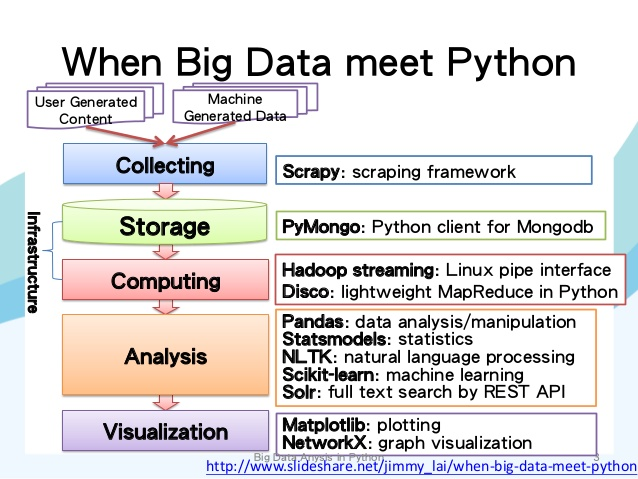
\includegraphics[width=0.99\linewidth]{flowchart}

\end{figure}

\end{frame}
%===========================================================%
\begin{frame}
	\frametitle{Continuum Analytics’ Anaconda}
	\begin{figure}
\centering
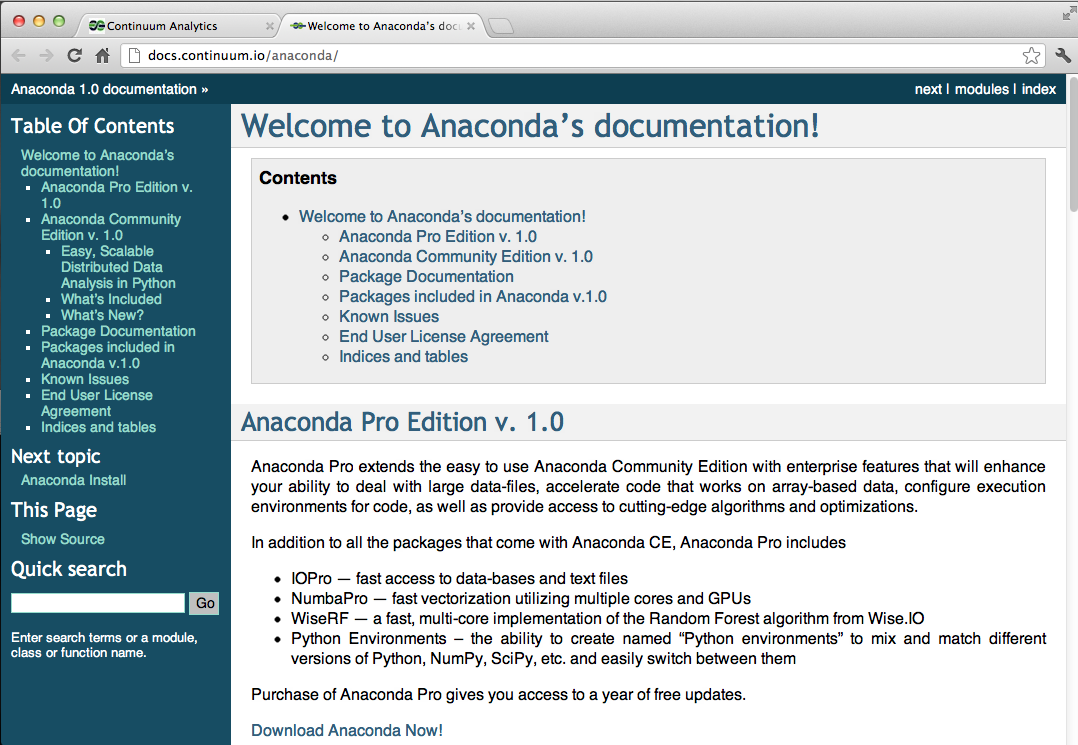
\includegraphics[width=1.0\linewidth]{anaconda.png}

\end{figure}

\end{frame}
%===========================================================%
\begin{frame}
\frametitle{Continuum Analytics’ Anaconda}
\large
\begin{itemize}
\item Anaconda, a free product of Continuum Analytics (www.continuum.io), is a virtually complete scientific
stack for Python. 
\item It includes both the core Python interpreter and standard libraries as well as most
modules required for data analysis. 

\end{itemize}
\end{frame}
%===========================================================%
\begin{frame}
\frametitle{Continuum Analytics’ Anaconda}
\large
	\begin{itemize}
\item Anaconda is free to use and modules for accelerating the performance
of linear algebra on Intel processors using the \textbf{Math Kernel Library} (MKL) are available (free to
academic users and for a small cost to non-academic users). 
\item Continuum Analytics also provides other
high-performance modules for reading large data files or using the GPU to further accelerate performance
for an additional, modest charge. 
	\end{itemize}

\end{frame}
%===========================================================%
\begin{frame}[fragile]
\frametitle{Installing Anaconda}
Most importantly, installation is extraordinarily easy onWindows, Linux
and OS X. Anaconda is also simple to update to the latest version using
\begin{framed}
\begin{verbatim}
conda update conda
conda update anaconda
\end{verbatim}
\end{framed}
\end{frame}
%===========================================================%
\begin{frame}
\frametitle{NumPy and SciPy}

\begin{itemize}
\item \textbf{NumPy} provides a set of array and matrix data types which are essential for statistics and econometrics.

\item \textbf{SciPy} contains a large number of routines needed for analysis of data.The most important include a wide
range of random number generators, linear algebra routines and optimizers. 

\item Remark: SciPy depends on NumPy.

\item More on them later.
\end{itemize}
\end{frame}
%===========================================================%
\begin{frame}
\frametitle{IPython}
IPython provides an interactive Python environment which enhances productivity when developing code
or performing interactive data analysis.
\end{frame}
%===========================================================%
\begin{frame}
	
	\begin{figure}
\centering
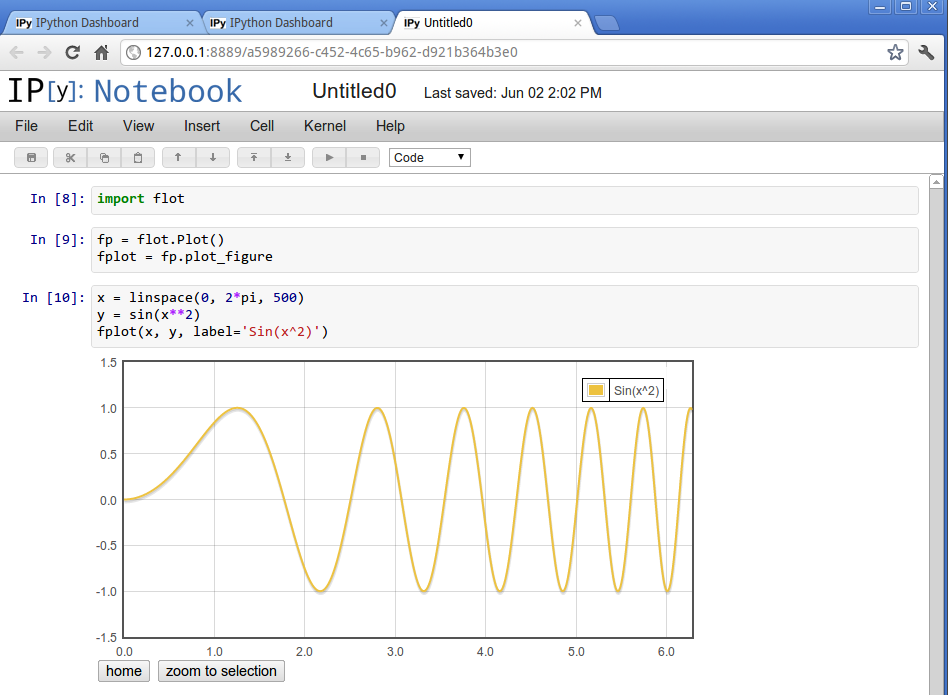
\includegraphics[width=0.9\linewidth]{vk2Q6}

\end{figure}

\end{frame}
%===========================================================%

\begin{frame}
	\textbf{Ipython Notebook / Jupyter}
	\vspace{-0.4cm}
	\begin{figure}
\centering

\includegraphics[width=1.0\linewidth]{jupyter}

\end{figure}

\end{frame}
	
\begin{frame}
	\begin{figure}
\centering
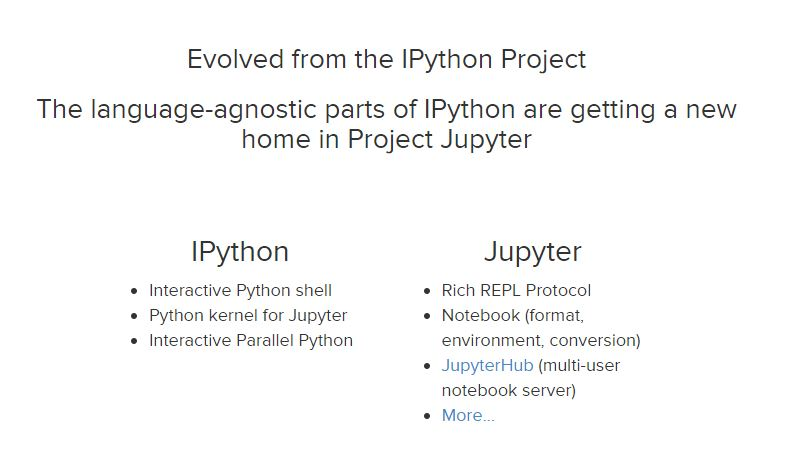
\includegraphics[width=1.0\linewidth]{jupytersiteinfo}

\end{figure}

\end{frame}
\begin{frame}
	Markdown is a text-to-HTML conversion tool for web writers. Markdown allows you to write using an easy-to-read, easy-to-write plain text format, then convert it to structurally valid XHTML (or HTML).
	\begin{figure}
\centering
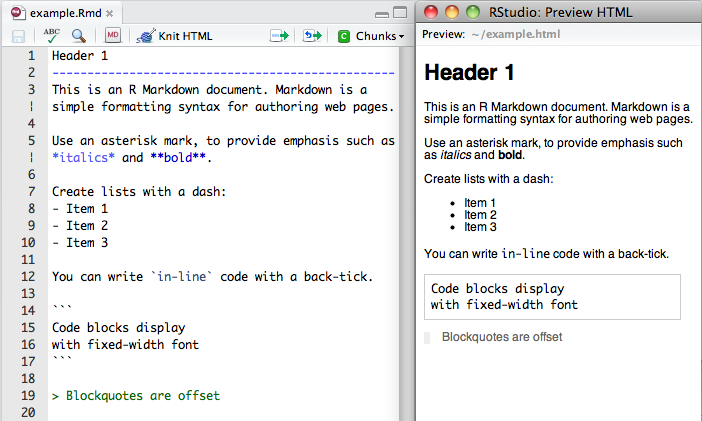
\includegraphics[width=0.85\linewidth]{markdownOverview}

\end{figure}

\end{frame}
%===========================================================%
\begin{frame}
\frametitle{matplotlib and seaborn}
\large
	\vspace{-0.4cm}
\textbf{Graphics Packages}
\begin{itemize}
\item \textbf{matplotlib} provides a plotting environment for 2D plots, with limited support for 3D plotting. 
\item \textbf{seaborn} is
a Python package that improves the default appearance of matplotlib plots without any additional code.
\end{itemize}

\end{frame}
%===========================================================%
\begin{frame}
\frametitle{pandas}
\Large
\begin{itemize}
\item 	\textit{pandas} is a high-performance module that provides a comprehensive set of structures for working with
data. 
\item \textit{pandas} excels at handling structured data, such as data sets containing many variables, working with
missing values and merging across multiple data sets. 
\end{itemize}
\end{frame}
%===========================================================%

%===========================================================%
\begin{frame}
	\large
	\frametitle{pandas}	
	\large
	\begin{itemize}
	
	\item While extremely useful, \textit{pandas} is not an essential component of the Python scientific stack unlike NumPy, SciPy or matplotlib, and so while \textit{pandas} doesn’t
	make data analysis possible in Python, it makes it much easier. \item \textit{pandas} also provides high-performance,
	robust methods for importing from and exporting to a wide range of formats.
	\item - example \texttt{read.csv()}
	\end{itemize}
\end{frame}
\begin{frame}
%=============================================================== %	
	\begin{figure}


\includegraphics[width=0.5\linewidth]{cythonlogo}

\end{figure}

\begin{figure}
\centering
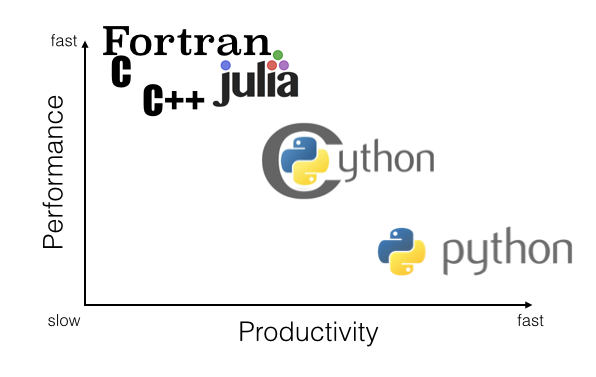
\includegraphics[width=0.7\linewidth]{cython_vs_chart}

\end{figure}

\end{frame}
%===========================================================%
\begin{frame}
	
	\large
\frametitle{Performance Modules : Cython and Numba}
A number of modules are available to help with performance. These include Cython and Numba.

\begin{description}
	\item[Cython] Cython
	is a Python module which facilitates using a simple Python-derived creole to write functions that can be
	compiled to native (C code) Python extensions. 
	
	
	\item[Numba] 
	Numba uses a method of just-in-time compilation to
	translate a subset of Python to native code using \textit{Low-Level Virtual Machine} (LLVM).
\end{description} 

\end{frame}

%=======================================================================%
\end{document}